\subsection*{\center Ejercicio 6. Teoría de la Empresa}
\vspace{1cm}

\begin{enumerate}[\large\bfseries 1.]

    %--------------------1.
    \item \textbf{Asignación de un recurso entre dos actividades}\\\\
    
    \begin{tcolorbox}[colframe=white]
	\begin{center}
	    \begin{tabular}{||ccc||c||ccc||}
		\hline
		$ProdMarg_O$&$PromProd_O$&$q_O$ (Tm)&Flota&$q_E$(Tm)&$PromProd_E$&$ProdMarg_E$\\	
		\hline
		 0&0&0&0&0&0&0\\
		 100&100&100&1&130&130&130\\
		 100&100&200&2&240&120&110\\
		 100&100&300&3&330&110&90\\
		 80&85&380&4&400&100&70\\
		 \hline
	    \end{tabular}
	\end{center}
    \end{tcolorbox}

	\begin{multicols}{2}
	    \begin{center}
		\begin{tikzpicture}[scale=1.15]
		    % abscisa y ordenada
		    \tkzInit[xmax= 5,xmin=0,ymax=500,ymin=0,ystep=100]
		    \tiny\tkzLabelX[opacity=0.4,step=1, orig=false]
		    \tiny\tkzLabelY[opacity=0.4,step=1, orig=false]
		    % label x, f(x)
		    \tkzDrawX[opacity= 1,label=Labor, right=.1]
		    \tkzDrawY[opacity= 1,label=Produción, below = -.5]
		    %dominio y función
		    \draw[step=1cm,black,very thin,opacity=.05] (0,0) grid (5.5,5.5);
		    \filldraw[black](0,0)node[below left]{$(0,0)$} circle (1.5pt);

		    \node at (2.5,6.5) {\textbf{Curvas de producto total, marginal y medio (E)}};

		    \filldraw[red](1,1.3)node[left]{$(1,130)$} circle (1.5pt);
		    \filldraw[red](2,1.1)node[below left]{$(2,110)$} circle (1.5pt);
		    \filldraw[red](3,0.9)node[below left]{$(3,90)$} circle (1.5pt);
		    \filldraw[red](4,0.7)node[below left]{$(4,70)$} circle (1.5pt);

		    \draw[red](0,0)..controls(1,1.55)..(2,1.1);
		    \draw[red](2,1.1)..controls(3,.9)..(4,0.7)node[below right]{$ProdMarg_E$};

		    \filldraw[green](2,2.4)node[above left]{$(2,240)$} circle (1.5pt);
		    \filldraw[green](3,3.3)node[above left]{$(3,330)$} circle (1.5pt);
		    \filldraw[green](4,4)node[above left]{$(4,400)$} circle (1.5pt);

		    \draw[green](0,0)..controls(1.3,2)and(3.5,4)..(5,4.5);
		    \draw[green](5.1,4.6)node[above]{$Producción E$};


		    \filldraw[blue](1,1.3)node[above right]{$(1,130)$} circle (1.5pt);
		    \filldraw[blue](2,1.2)node[above right]{$(2,120)$} circle (1.5pt);
		    \filldraw[blue](3,1.1)node[above right]{$(3,110)$} circle (1.5pt);
		    \filldraw[blue](4,1)node[above right]{$(4,100)$} circle (1.5pt);

		    \draw[blue](0,0)..controls(1,1.5)..(2,1.2);
		    \draw[blue](2,1.2)..controls(3,1.1)..(4,1)node[below right]{$PromProd_E$};
		    \draw[blue](5.1,4.25);
		\end{tikzpicture}
	    \end{center}

	    \begin{center}
		\begin{tikzpicture}[scale=1.15]
		    % abscisa y ordenada
		    \tkzInit[xmax= 5,xmin=0,ymax=500,ymin=0,ystep=100]
		    \tiny\tkzLabelX[opacity=0.4,step=1, orig=false]
		    \tiny\tkzLabelY[opacity=0.4,step=1, orig=false]
		    % label x, f(x)
		    \tkzDrawX[opacity= 1,label=Labor, right=.1]
		    \tkzDrawY[opacity= 1,label=Produción, below = -.5]
		    %dominio y función
		    \draw[step=1cm,black,very thin,opacity=.05] (0,0) grid (5.5,5.5);

		    \node at (2.5,6.5) {\textbf{Curvas de producto total, marginal y medio (O)}};

		    \filldraw[black](0,0)node[below left]{$(0,0)$} circle (1.5pt);

		    \filldraw[red](1,1)node[left]{$(1,100)$} circle (1.5pt);
		    \filldraw[red](2,1)node[below left]{$(2,100)$} circle (1.5pt);
		    \filldraw[red](3,1)node[below left]{$(3,100)$} circle (1.5pt);
		    \filldraw[red](4,.8)node[below left]{$(4,80)$} circle (1.5pt);

		    \draw[red](0,0)..controls(1,1.2)..(2,1);
		    \draw[red](2,1)..controls(3,1.05)..(4,.8)node[below right]{$ProdMarg_O$};

		    \filldraw[green](2,2)node[below right]{$(2,200)$} circle (1.5pt);
		    \filldraw[green](3,3)node[below right]{$(3,300)$} circle (1.5pt);
		    \filldraw[green](4,3.8)node[below right]{$(4,380)$} circle (1.5pt);

		    \draw[green](0,0)..controls(1.9,1.75)and(3,3.5)..(5,4.3);
		    \draw[green](5.1,4.48)node[above]{$Producción O$};

		    \filldraw[blue](2,1)node[above]{$(2,100)$} circle (1.5pt);
		    \filldraw[blue](3,1)node[above]{$(3,100)$} circle (1.5pt);
		    \filldraw[blue](4,.85)node[above]{$(4,85)$} circle (1.5pt);

		    \draw[blue,opacity=.7](0,0)..controls(1,1.2)..(2,1);
		    \draw[blue,opacity=.7](2,1)..controls(3,1.05)..(4,.85)node[right]{$PromProd_O$};
		    \draw[blue](5.1,4.25);
		\end{tikzpicture}
	    \end{center}
	\end{multicols}
	    \vspace{1cm}

	\begin{enumerate}[\bfseries a)]

	    %----------a)
	    \item Utilizando la teoría económica, explíquele a su armador cuál es la distribución óptima entre ambos bancos de pesca.\\\\
		A pesar de que los gráficos nos dan un panorama general, analizaremos en particular los barcos, como recursos que no son perfectamente divisibles. La teoría económica es la siguiente:
		\begin{center}
		    $"$ Para repartir eficientemente un recurso entre diferentes actividades productivas consiste en asignar cada unidad del recurso a la actividad productiva en la que su producto marginal es el más alto  (Robert Frank) $"$.
		\end{center}
		Ahora bien para hallar la distribución óptima entre los dos barcos de pesca simplemente se deducirá a la mayor distribución de su producción total, en este caso 440 toneladas (100 de cada uno de los barcos del Oeste y 120 de los barcos del lado Este.) como se verá en la siguiente tabla.\\\\
	    \begin{tcolorbox}[colframe=white]
		\begin{center}
		    \begin{tabular}{|cc||c|}
			\hline
			barco Este&Barco Oeste&cantidades producidas\\
			\hline
			4&0&400\\
			3&1&430\\
			\hline
			2&2&440\\
			\hline
			1&3&430\\
			0&4&380\\
			\hline
		    \end{tabular}
		\end{center}
	    \end{tcolorbox}
	    \vspace{1cm}

	    %---------b)
	    \item Hágale ver cuál es su error al tomar la productividad media tanto al principio cuando quería mandar todos los barcos hacia Rande, como después que quería mandar un barco más a Rande.\\\\
	    Sabiendo que los costes de mandar a cualquiera de los dos bancos de pesca son iguales , Supongamos que mandamos solamente dos barcos hacia Rande, por lo tanto la captura media estará dado por 20 toneladas diarias, más que las capturas del otro extremo. A esto observe que si mandamos un tercer barco a Rande, la contribución a la cantidad total será de 90 toneladas, es decir, la diferencia entre 330 Toneladas y 240 Toneladas. Algo muy importante es el hecho de que el tercer barco que pesta en Rande captura del pescado que habría sido capturado por los dos primeros.\\
Por lo tanto el coste de oportunidad de mandar un tercer barco a Rande son las 100 toneladas que ya no se capturaran en las Islas Cíes, como se verá a continuación:\\

    	    \begin{tcolorbox}[colframe=white]
	    \begin{center}
		\begin{tabular}{ccc}
		    B(Rande)&>&C(Istas Cíes)\\
		    \hline
		    90&$\ngtr$&100\\
		\end{tabular}
	    \end{center}
	    \end{tcolorbox}
	    Análogamente, si enviamos un cuarto barco a Rande, el coste de oportunidad será de $100$  y el beneficio solo de 70 toneladas.\\\\

	\end{enumerate}

    %--------------------2.
    \item \textbf{La decisión de producción de la empresa basadas en la productividad de los inputs productivos deben coincidir con la decisión de producción de la empresa basadas en los costes de producir.}\\

	\begin{enumerate}[\bfseries 2.1]

	    %----------2.1)
	    \item \textbf{La decisión de producción de la empresa basadas en la productividad de los inputs productivos.}\\\\
		Para poder emplear la Regla de Decisión Racional y estudiar las decisiones marginales de María como empresaria maximizadora de beneficios. En particular, debemos que tomar en cuenta los costes implícitos. Para ello planteamos la pregunta siguiente sabiendo que $X = $ Ir a pescar, $Y = $ Ir a la tienda,
		\begin{tcolorbox}[colframe=white]
		    \begin{center}
			¿Debo realizar la acción $X$ en lugar de su mejor acción alternativa $Y$?.
		    \end{center}
		\end{tcolorbox}

		Para ello realizaré la acción $X$, en lugar de su mejor acción alternativa $Y$, cuando los beneficios de realizar la acción $X$, en lugar de la mejor alternativa $Y$, sean mayores que sus costes, es decir,
		$$B(X)+C(Y) = B(X \; vx. \; Y) > C(X \; vs. \; Y = C(X)+B(Y)$$
		en caso contrario no realizaré dicha acción.\\

		\begin{center}
		    \begin{tabular}{ccccc}
			Hr&Cant. de pescado (kg)&Trabajar en tienda&Beneficio de Pescar (p=2.5)&$B_{Marg}$ de pescar\\
			\hline\\
			     0&0&0&0&0\\
			     1&10&12&25&25\\
			     2&18&12&45&20\\
			     3&24&12&60&15\\
			     4&28&12&70&10\\
			     5&30&12&75&5\\
		    \end{tabular}
		\end{center}
		\vspace{.5cm}

		Luego $B(X)$ será  el beneficio marginal de pescar una hora más, y  el coste de oportunidad estará compuesto por el coste de ir a pescar más el costo implícito de alquilar la caña y el sedal por todo un día ($B(Y) = 24/12 = 2$), es decir, $C(X)+B(Y)$. Así, la Regla de decisión Racional vendrá dado por:\\

		\begin{tcolorbox}[colframe=white]
		    \begin{center}
			\begin{tabular}{c|rcl}
			    hrs&B(X vs. Y)&>&C(X vs. Y)\\\\
			    \hline\\
			       1&25&>&14 = 12+2\\
			       2&20&>&14\\
			       3&15&>&14\\
			       4&10&<&14\\
			\end{tabular}
		    \end{center}
		\end{tcolorbox}

		Y por lo tanto la decisión óptima que deberá realizar María será la de ir a pescar 3 horas y trabajar en la tienda 2 horas.\\\\

	    %---------2.2)
	    \item \textbf{La decisión de producción de la empresa basadas en los costes de producir.}\\\\

		\begin{enumerate}[\bfseries a)]

		    %----------a)
		    \item \textbf{Tabla de costes de la explotación pesquera para cada nivel de producción}\\\\
		    \begin{tcolorbox}[colframe=white]
			\begin{center}
			    \begin{tabular}{|c|c|c|c|c|c|c|c|}
				     \hline
				Horas&Cantidad de &Coste&Coste&Coste&CV&CT&Coste\\
				     &pescado (kilos)&fijo&variable&total&medio&medio&marginal\\
				     \hline
				     0&0&12&0&12&-&-&-\\
				     1&10&12&12&24&1.2 &2.4 &1.2\\
				     2&18&12&24&28&1.33&1.56&1.5\\
				     3&24&12&36&48&1.5 &2   &2\\
				     4&28&12&48&60&1.71&2.14&3\\
				     5&30&12&60&72&2   &2.4 &6\\
				     \hline
			    \end{tabular}
			\end{center}
		    \end{tcolorbox}
		    \vspace{1cm}

		    %---------b)
		    \item \textbf{En el corto plazo ¿cuál es el precio de beneficio cero?, ¿cuál es el precio de cierre de la empresa?}\\\\
			El precio de beneficio está dado por 2 Euros, porque  el beneficio será nulo como bien indica el nombre, es decir, el precio cubrirá  los costos variables y los costes fijos.
			El precio de cierre viene dado por 1.2 Euros, ya que se recuperará sólo los costes variables.\\\\
			

		    %---------c)
		    \item \textbf{Represente gráficamente la curva de coste total medio (CTMe), coste variable medio (CVMe) y coste marginal (CMg) de la empresa de pesca. En el mismo gráfico represente la curva de oferta a corto plazo e indique el precio de cierre y el precio de beneficio cero.}\\\\

		    \begin{center}
			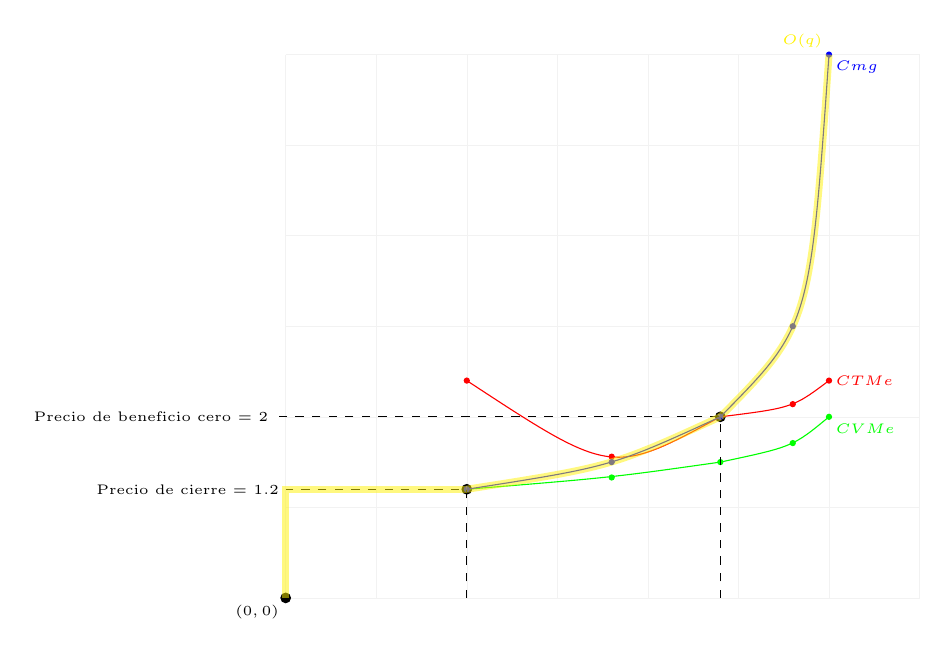
\begin{tikzpicture}[scale=1.15]
			    % abscisa y ordenada
			    \tkzInit[xmax= 35,xmin=0,xstep=5,ymax=6,ymin=0,ystep=1]
			    \tiny\tkzLabelX[opacity=0.4,step=1, orig=false]
			    \tiny\tkzLabelY[opacity=0.4,step=1, orig=false]
			    % label x, f(x)
			    \tkzDrawX[opacity= 1,label=q (output por hora), right=.1]
			    \tkzDrawY[opacity= 1,label=Coste asignado a cada unidad producida, below = -.5]
			    %dominio y función
			    \draw[step=1cm,black,very thin,opacity=.05] (0,0) grid (7,6);
			    \filldraw[black](0,0)node[below left]{$(0,0)$} circle (1.5pt);

			    \filldraw[red](2,2.4) circle (.8pt);
			    \filldraw[red](3.6,1.56) circle (.8pt);
			    \filldraw[](4.8,2) circle (1.5pt);
			    \filldraw[red](5.6,2.14) circle (.8pt);
			    \filldraw[red](6,2.4) circle (.8pt);

			    \draw[red](2,2.4)..controls(3.6,1.35)..(4.8,2);
			    \draw[red](4.8,2)..controls(5.6,2.1)..(6,2.4)node[right]{$CTMe$};

			    \filldraw[](2,1.2) circle (1.5pt);
			    \filldraw[green](3.6,1.33) circle (.8pt);
			    \filldraw[green](4.8,1.5) circle (.8pt);
			    \filldraw[green](5.6,1.71) circle (.8pt);
			    \filldraw[green](6,2) circle (.8pt);

			    \draw[green](2,1.2)..controls(3.6,1.33)..(4.8,1.5);
			    \draw[green](4.8,1.5)..controls(5.6,1.67)..(6,2)node[below right]{$CVMe$};

			    \filldraw[blue](2,1.2) circle (.8pt);
			    \filldraw[blue](3.6,1.5) circle (.8pt);
			    \filldraw[blue](4.8,2) circle (.8pt);
			    \filldraw[blue](5.6,3) circle (.8pt);
			    \filldraw[blue](6,6) circle (.8pt);

			    \draw[blue](2,1.2)..controls(3.6,1.45)..(4.8,2);
			    \draw[blue](4.8,2)..controls(5.79,3)..(6,6)node[below right]{$Cmg$};

			    \draw[dashed](2,0)--(2,1.2)--(0,1.2)node[left]{Precio de cierre = $1.2$};
			    \draw[dashed](4.8,0)--(4.8,2)--(-0.12,2)node[left]{Precio de beneficio cero = 2 };
			    %curva de oferta
			    \draw[line width = 0.9mm, yellow, opacity=.5](0,0)--(0,1.2)--(2,1.2);
			    \draw[line width = 0.9mm, yellow, opacity=.5](2,1.2)..controls(3.6,1.45)..(4.8,2);
			    \draw[line width = 0.9mm, yellow, opacity=.5](4.8,2)..controls(5.79,3)..(6,6);
			    \draw[yellow](6,6)node[above left]{$O(q)$};

			\end{tikzpicture}
		    \end{center}
		    \vspace{1cm}

		    %---------d)
		    \item \textbf{¿Cuántos kilos de pescado debería pescar la empresa de María si el precio del kilo de pescado es de 2,5 euros?.}\\\\
			Ya que estamos en una competencia perfecta se tiene que  el ingreso marginal es constante y está dada por $\overline{p}$. \\ 
			Luego, Aplicando la regla de decisión racional, podremos seguir pescando siempre y cuando el ingreso marginal sea mayor al costo marginal.\\\\


		    \begin{center}
			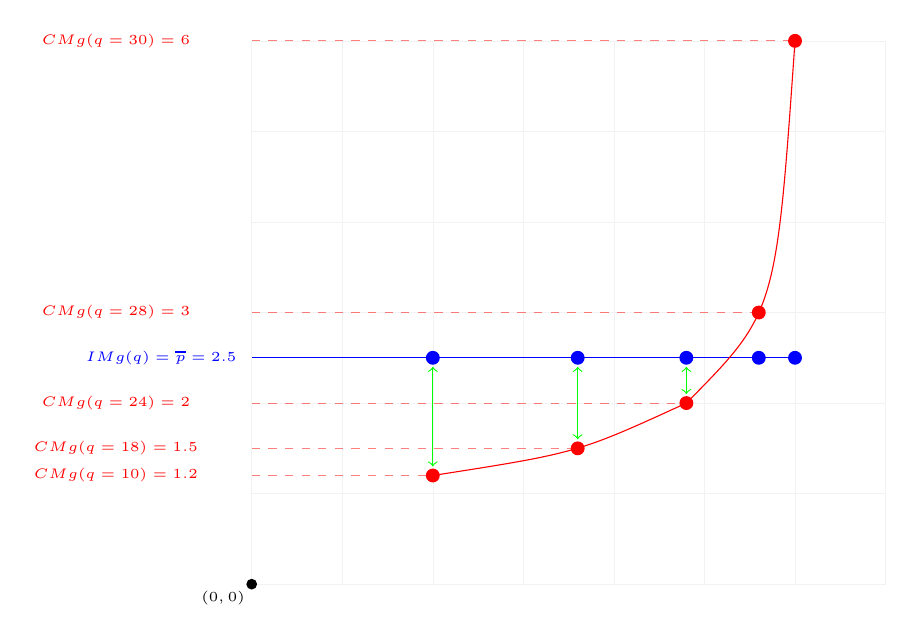
\begin{tikzpicture}[scale=1.15]
			    % abscisa y ordenada
			    \tkzInit[xmax= 35,xmin=0,xstep=5,ymax=6,ymin=0,ystep=1]
			    \tiny\tkzLabelX[opacity=0.4,step=1, orig=false]
			    \tiny\tkzLabelY[opacity=0.4,step=1, orig=false]
			    % label x, f(x)
			    \tkzDrawX[opacity= 1,label=q, right=.1]
			    \tkzDrawY[opacity= 1,label=Precio-Costo, below = -.5]
			    %dominio y función
			    \draw[step=1cm,black,very thin,opacity=.05] (0,0) grid (7,6);
			    \filldraw[black](0,0)node[below left]{$(0,0)$} circle (1.5pt);

			    \draw[blue](-1,2.5)node[]{$IMg(q) = \overline{p} =  2.5$};
			    \draw[blue](0,2.5)--(6,2.5);
			    \filldraw[blue](2,2.5) circle (2pt);
			    \filldraw[blue](3.6,2.5) circle (2pt);
			    \filldraw[blue](4.8,2.5) circle (2pt);
			    \filldraw[blue](5.6,2.5) circle (2pt);
			    \filldraw[blue](6,2.5) circle (2pt);


			    \draw[red](-1.5,1.2)node[]{$CMg(q=10) = 1.2$};
			    \filldraw[red](2,1.2) circle (2pt);
			    \draw[red, dashed, opacity = .5](0,1.2)--(2,1.2);

			    \draw[red](-1.5,1.5)node[]{$CMg(q=18) = 1.5$};
			    \filldraw[red](3.6,1.5) circle (2pt);
			    \draw[red, dashed, opacity = .5](0,1.5)--(3.6,1.5);

			    \draw[red](-1.5,2)node[]{$CMg(q=24) = 2$};
			    \filldraw[red](4.8,2) circle (2pt);
			    \draw[red, dashed, opacity = .5](0,2)--(4.8,2);

			    \draw[red](-1.5,3)node[]{$CMg(q=28) = 3$};
			    \filldraw[red](5.6,3) circle (2pt);
			    \draw[red, dashed, opacity = .5](0,3)--(5.6,3);

			    \draw[red](-1.5,6)node[]{$CMg(q=30) = 6$};
			    \filldraw[red](6,6) circle (2pt);
			    \draw[red, dashed, opacity = .5](0,6)--(6,6);

			    \draw[green,<->](2,1.3)--(2,2.4);
			    \draw[green,<->](3.6,1.6)--(3.6,2.4);
			    \draw[green,<->](4.8,2.1)--(4.8,2.4);


			    \draw[red](2,1.2)..controls(3.6,1.45)..(4.8,2);
			    \draw[red](4.8,2)..controls(5.79,3)..(6,6);

			\end{tikzpicture}
		    \end{center}
		    
		    \begin{tcolorbox}[colframe=white]
			\begin{center}
			    \begin{tabular}{c|rcl}
				Cantidad&Img&>&Cmg\\\\
				    \hline\\
				    10&2.5&>&1.2\\
				    18&2.5&>&1.5\\
				    24&2.5&>&2\\
				    28&2.5&<&3\\
			    \end{tabular}
			\end{center}
		    \end{tcolorbox}
		    \vspace{.5cm}
		    Por lo tanto María deberá producir 24 kilos de pescado a un precio de 2.5 euros.\\\\

		    %---------e)
		    \item  \textbf{Compare la respuesta del apartado d) con el que obtuvo en el Ejercicio 2.1.}\\\\
			Efectivamente la decisión de horas de trabajo de María coincide con la decisión productiva de la empresa de María ya que no podremos separar al empresario como consumidor a y a la empresa como maximizadora de beneficios por el hecho de que no se cumple el supuesto de $"$No incertidumbre $"$, es decir, María se encuentra en una disyuntiva entre ir a pescar o atender una tienda y por ende cae en la incertidumbre de arriesgar a constituir una empresa o no.\\\\


		\end{enumerate}


	\end{enumerate}

\end{enumerate}
